\documentclass[a4paper,12pt]{article}
\usepackage[T1]{fontenc}
\usepackage{imakeidx}
\usepackage{graphicx}
%\makeindex[columns=3, title=Alphabetical Index, intoc]

\begin{document}
\textbf{PC components}
\tableofcontents

\section{Introduction}
In this document,we explain several parts \index{Introduction} of the Personal Computer
and every one of them should appear in the Index\index{Introduction} above.

\clearpage

\section{Central Processor Unit}
This section\index{CPU, Processor} is meant to illustrate the main component of a PC 
which is the Processor usually addressed as CPU.
This is the piece of hardware that phisically executes \emph{software} instructions one at at time.
Without this component there is no chance to have a running computer. It belongs to the bare minimum set of 
components that you need to have if you want to have something that you can call a PC.

\subsection{internal CPU structure and low level language}
Inside of the CPU there is a set of \emph{registers} available for software developers to use.
Usually software developer write their code in a \emph{high level language} such as C++, Python, Java, etc.
The reason they're called high level languages is because there is a high level of abstraction from the processor
language level which is usually called assembly language (like 8086 or Motorola M68000)

Every \emph{core} of the processor executes one piece of code properly \emph {compiled} in the low level architecture language by the compiler.

The reason why today we have usually more than one core is to allow concurrency which means more than one piece of
code executed at a time. This is achieved by developers by doing concurrent programming which essentially is all about
writing a software thinking at every instruction which process is executing it, so we'll find in the code checks like
\[if (pid==0)\]
where $pid$ is the ID of the $\bf process$ executing the "if" instruction which returns true only when the $\bf process$ hasn't  got any \emph{sons}. If it returns false then we're facing the father process, which usually is the process where the son has been generated from but
we'll go more in depht on this later on

%Let $D$ be a subset of $\bf R$ and let
%$f \colon D \to \mathbf{R}$ be a real-valued function on
%$D$. The function $f$ is said to be \emph{continuous} on
%$D$ if, for all $\epsilon > 0$ and for all $x \in D$,
%there exists some $\delta > 0$ (which may depend on $x$)
%such that if $y \in D$ satisfies
%\[ |y - x| < \delta \]
%then
%\[ |f(y) - f(x)| < \epsilon. \]

%One may readily verify that if $f$ and $g$ are continuous
%functions on $D$ then the functions $f+g$, $f-g$ and
%$f.g$ are continuous. If in addition $g$ is everywhere
%non-zero then $f/g$ is continuous.

\clearpage

\section{Hard Drive}
The hard drive popularly called HDD that stands for \emph{hard disk drive}, is the part of the computer where data is stored.We do not lose data inside of an HDD when this is disconnected,for that reason is considered to be one of the main component when you're thinking about storing data.Files and programs are stored at its inside which can be executed. Some of the hard drives are connected with technologies called : IDE/ATA, Serial ATA, and SCSI.

\subsection{types of hard drive}
There are SSD\index{SSD} drives and old fashion ones

\subsubsection{SSD}
It stands for solid state drive and does not have any moving part inside of it that in the old days we would have seen to be used in order to store phisically data.Essentially it is a flash memory which reminds of what has been already used in USB pen drives.

\subsubsection{Old Fashion ones}
These have a moving part inside required to store data and can be damaged more easily if there is a power outage.
In order to store sequences of 0 and 1, there is a magnetic moving arm capable of hitting the disk thousand of times per second.Every bit is made by a particular molecular sequence.
\clearpage

\section{Memory}

Usually addressed as RAM (stands for Random Access Memory), made in silicon technology it is used to store temporary data for the operative system to function properly. It's usually installed in modules each one of each provides a specific capacity.

Every bit is stored thanks to a component called Flip-Flop. It is usually organized as a matrix of Flip-Flop JK every one of each stores 1 bit only. Every Flip Flop can be accessed thanks to the presence of two decoders as shown in figure :
 
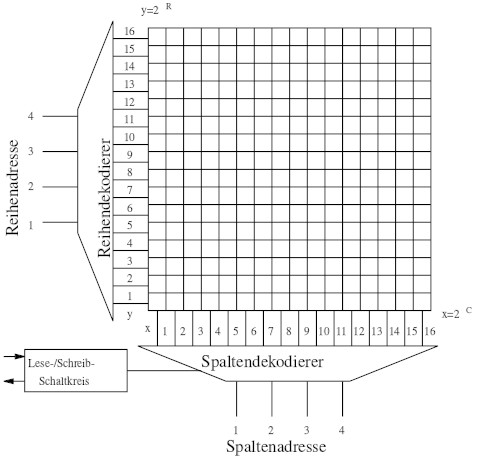
\includegraphics[width=9cm]{./DRAM-02.jpg}

The module shown in picture is one of the most essential and primitive blocks in a RAM slots and stores just 256 bits, namely 32 bytes. 
The word Random now makes sense. By looking at the two decoders in pictures we can now understand what Random means. It means that no matter which block of memory we want to have access at, the time needed to read/write that block will be the same. That's why it's called Random. You can choose a Random point in a memory slot and this won't affect in any way the time needed to access that particular portion of memory
\subsection{types of Memory}

We have SDRAM\index{SDRAM}, SO-DIMM\index{SO-DIMM} and SERVER RAM.

\subsubsection{SERVER RAM}
This ram is mission critical. It's mainly used when a stable environment is required such the one offered by Windows Vista (the only Operative System that has ever achieved \emph{Deadlock Prevention} algorithm).
Like Windows Vista this RAM suffers from low speed issued. Vista is because of the Deadlock Detection strategy. Server RAM because of the bit parity check. In both cases the user experience would be horrible. This is why these two things should be only operating in Server side where processes have to be checked and memory integrity needs to be ensured


\section{Power Supply Unit}

A PC power supply, also known as a computer power supply, is used to power computers. The main alternating current is transformed into the lower DC voltages required in the computer. It is designed as a switching power supply. On the PC, it is built into the case.  Laptops and some miniature PCs have external power supplies with similar characteristics. Built-in power supplies also contain fans which, in addition to self-cooling, serve in whole or in part to cool the components installed in the computer case. 

\section{GPU}
This is the graphic processor unit thas performs graphic operations or floating point operations to make the CPU life easier in 3D applications or videogames.  Something the GPU takes care of is the antialiasing( a technique to smoothen the border of an object to make it look more realistic). Every graphic board has a GPU and many setups today include onboard graphics already.

\printindex



\end{document}
